\documentclass[conference]{IEEEtran}
\IEEEoverridecommandlockouts
\usepackage[letterpaper, 
            top=1in,        % 72pt top margin (first page)
            bottom=0.75in,  % 54pt bottom margin
            left=0.75in,    % 54pt left margin
            right=0.75in]   % 54pt right margin
            {geometry}
\usepackage{cite}
\usepackage{amsmath,amssymb,amsfonts}
\usepackage{algorithmic}
\usepackage{graphicx}
\usepackage{textcomp}
\usepackage{orcidlink}
\usepackage{xcolor}
\usepackage{comment}
\def\BibTeX{{\rm B\kern-.05em{\sc i\kern-.025em b}\kern-.08em
    T\kern-.1667em\lower.7ex\hbox{E}\kern-.125emX}}




%%%
\usepackage{xcolor}
\usepackage{soul}
% 1. Define custom soft/pastel marker colors (RGB format)
\definecolor{markergreen}{RGB}{204, 255, 204}
\definecolor{markerred}{RGB}{255, 204, 204}
\definecolor{markeryellow}{RGB}{255, 255, 204}
% 2. Create custom shortcut commands for quick highlighting
\newcommand{\hlgreen}[1]{{\sethlcolor{markergreen}\hl{#1}}}
\newcommand{\hlred}[1]{{\sethlcolor{markerred}\hl{#1}}}
\newcommand{\hlyellow}[1]{{\sethlcolor{markeryellow}\hl{#1}}}
%%% 
\setlength{\parindent}{0pt}
\begin{document}

\title{Adaptive Process Noise Estimation in Sim2Real Frameworks: A Comparative Analysis Across Nonlinear Kalman Filters}

\author{\IEEEauthorblockN{1\textsuperscript{st} Barak Diker~\orcidlink{0009-0003-4551-3061}}
\IEEEauthorblockA{\textit{Hatter Dept of Marine Technologies} \\
\textit{Charney School of Marine Sciences}\\
\textit{University of Haifa}\\
Haifa, Israel \\
bdiker01@campus.haifa.ac.il}
\and
\IEEEauthorblockN{2\textsuperscript{nd} Gal Versano~\orcidlink{0009-0007-7766-2511}}
\IEEEauthorblockA{\textit{Hatter Dept of Marine Technologies} \\
\textit{Charney School of Marine Sciences}\\
\textit{University of Haifa}\\
Haifa, Israel \\
gversano@staff.haifa.ac.il}
\and
\IEEEauthorblockN{3\textsuperscript{rd} Nadav Cohen~\orcidlink{0000-0002-8249-0239}}
\IEEEauthorblockA{\textit{Hatter Dept of Marine Technologies} \\
\textit{Charney School of Marine Sciences}\\
\textit{University of Haifa}\\
Haifa, Israel \\
ncohe140@campus.haifa.ac.il}
\and
\IEEEauthorblockN{4\textsuperscript{th} Amit Levy~\orcidlink{0009-0009-8703-5807}}
\IEEEauthorblockA{\textit{Hatter Dept of Marine Technologies} \\
\textit{Charney School of Marine Sciences}\\
\textit{University of Haifa}\\
Haifa, Israel \\
alevy02@campus.haifa.ac.il}
\and
\IEEEauthorblockN{5\textsuperscript{th} Itzik Klein~\orcidlink{0000-0001-7846-0654}}
\IEEEauthorblockA{\textit{Hatter Dept of Marine Technologies} \\
\textit{Charney School of Marine Sciences}\\
\textit{University of Haifa}\\
Haifa, Israel \\
kitzik@univ.haifa.ac.il}
}

\maketitle

\begin{abstract}
% This document is a model and instructions for \LaTeX.
% This and the IEEEtran.cls file define the components of your paper [title, text, heads, etc.]. *CRITICAL: Do Not Use Symbols, Special Characters, Footnotes, 
% or Math in Paper Title or Abstract.
Accurate underwater navigation is challenging due to the unavailability of GNSS signals and time-varying uncertainties in inertial and Doppler velocity log measurements. Several works have investigated the contribution of neural-aided adaptive process noise covariance to positioning accuracy, yet without a common ground for comparison and analysis. To bridge this gap, we benchmark three nonlinear Kalman filter variants under an adaptive process noise estimation mechanism designed using a Sim2Real training approach. Through this comparative benchmarking framework and using 80.8 minutes of real-world autonomous underwater vehicles trajectories, we demonstrate that the Sim2Real adaptive invariant Kalman filter outperforms the baseline Sim2Real adaptive extended Kalman filter by 57.2\%. These results provide practical guidance for selecting a nonlinear filtering approach in Sim2Real strategies, and highlight the benefit of combining adaptive process noise estimation with invariant filtering for underwater navigation.
\end{abstract}
\begin{IEEEkeywords}
Kalman filter, Sensor fusion, Adaptive process noise, State estimation, Lie group.
\end{IEEEkeywords}
\section{Introduction}
\noindent Accurate underwater navigation is challenging because global navigation satellite system (GNSS) signals are unavailable below the water surface. Autonomous underwater vehicles (AUVs) must therefore rely on onboard sensor fusion, commonly combining inertial measurements with Doppler velocity log (DVL) observations, to estimate their position, velocity, and orientation. \\
\noindent Nonlinear Kalman filters, including the extended Kalman filter (EKF) \cite{10.5555/1594745,bar2011tracking}, unscented Kalman filter (UKF) \cite{wan2001unscented,simon2006optimal}, and right-invariant Kalman filter (RI-IKF) \cite{barrau2018invariant,barrau2017three,hartley2020contact}, provide established frameworks for inertial/DVL sensor fusion \cite{groves2013principles,klein2020continuous,damari2026ai,hu2025tightly,chen2024seamless}. Their performance, however, depends strongly on the process noise covariance matrix, which is commonly fixed and manually tuned. Because AUV dynamics, sensor characteristics, and environmental disturbances vary over time, a fixed process noise covariance may not adequately represent the uncertainty of the navigation model. \\
\noindent Adaptive Kalman filtering has been investigated extensively for INS/DVL navigation under uncertain and time-varying noise conditions. Existing methods include innovation-based covariance adaptation \cite{mohamed1999adaptive,magill1965optimal,meng2016covariance,mehra1972approaches}, recursive noise estimation \cite{gao2015adaptive}, online system noise covariance estimation \cite{wang2023system,kost2022measurement}, adaptive nonlinear filtering \cite{jin2023adaptive}, and variational Bayesian covariance estimation \cite{davari2019variational}. Robust adaptive filters have also been developed for complex underwater environments \cite{qian2023ins}. In parallel, invariant error formulations have been applied to SINS/DVL integration, including adaptive and robust variants designed to address inaccurate process and measurement noise covariances \cite{tang2023invariant,xu2024invariant}. \\
\noindent More recently, neural-aided approaches have been used to estimate time-varying inertial-noise parameters and adapt the process noise covariance online \cite{11361209,cohen2024inertial,diker2026neural,solodar2024vio}. However, existing studies generally employ different filtering formulations, datasets, sensor configurations, and adaptation mechanisms. Consequently, their reported improvements do not provide a common basis for determining how the underlying nonlinear filtering formulation influences the benefit obtained from adaptive process noise covariance estimation. \\
\noindent This paper provides a common-ground, real-world benchmark of the EKF, UKF, and RI-IKF and their neural-aided variants under identical conditions. All three variants employ the Sim2Real adaptive mechanism introduced in \cite{diker2026neural}, which combines neural inertial-noise estimation with innovation-based covariance adaptation. \\
\noindent \hlgreen{The Sim2Real approach utilizes domain randomization on simulated trajectories to train a noise-estimating neural network, enabling direct online deployment on unlabelled real-world data. Our evaluation reveals that the Neural-Aided RI-IKF leverages this adaptation most effectively, reducing mean position error} by 42.4\% and 57.2\% compared to the neural-aided UKF and EKF, respectively, thereby demonstrating a strong synergy between data-driven covariance estimation and Lie-group formulations. \\
\noindent The remainder of this paper is organized as follows. Section~\ref{sec:problem_formulation} introduces the EKF, UKF, and RI-IKF formulations. Section~\ref{sec:adaptive_covariance} describes the common adaptive covariance-estimation mechanism. Section~\ref{sec:results} presents the benchmark dataset, evaluated filtering approaches, and experimental results. Section~\ref{sec:conclusion} concludes the paper. \\
\section{Problem Formulation}
\label{sec:problem_formulation}
The inertial navigation equations expressed in the earth centered earth frame (ECEF) are \cite{titterton2004strapdown}.
\begin{equation}
  \label{dynamics_ode}
\begin{aligned}
&\dot{\boldsymbol{p}}_{eb}^{e} = \boldsymbol{v}_{eb}^{e} \\
&\dot{\boldsymbol{v}}_{eb}^{e} = \mathbf{C}_{b}^{e} \boldsymbol{f}_{ib}^{b}
- 2(\boldsymbol{\omega}_{ie}^{e})^{\wedge} \boldsymbol{v}_{eb}^{e}
+ \boldsymbol{g}_{ib}^{e} \\
&\dot{\mathbf{C}}_{b}^{e} = \mathbf{C}_{b}^{e}(\boldsymbol{\omega}_{ib}^{b})^{\wedge}
- (\boldsymbol{\omega}_{ie}^{e})^{\wedge} \mathbf{C}_{b}^{e}
\end{aligned}
\end{equation}
where the \(\boldsymbol{p}_{eb}^e\) and \(\boldsymbol{v}_{eb}^e\) are the position and velocity, respectively, of the body frame relative to ECEF frame resolved in ECEF frame. \(\boldsymbol{\omega}_{ib}^b\) and \(\boldsymbol{f}_{ib}^b\) are the angular velocity and the specific force vectors of body with respect to the inertial frame resolved in body frame, respectively, and \(\mathbf{C}_b^e\) is the rotation matrix from body frame to ECEF frame.
\subsection{Extend Kalman filter}
The error-state vector and the corresponding process-noise vector are defined as \cite{10.5555/1594745,groves2013principles}
\begin{equation}
  \label{ekf_state}
\delta \mathbf{x}_{\text{EKF}}
=
\begin{bmatrix}
\delta\boldsymbol{\phi}^b\\
\delta\boldsymbol{v}_{eb}^e\\
\delta\boldsymbol{p}_{eb}^e\\
\delta\boldsymbol{b}_g\\
\delta\boldsymbol{b}_a
\end{bmatrix}
\in\mathbb{R}^{15}
\qquad
\mathbf w
=
\begin{bmatrix}
\boldsymbol n_g\\
\boldsymbol n_a\\
\boldsymbol n_{b_g}\\
\boldsymbol n_{b_a}
\end{bmatrix}
\in\mathbb{R}^{12}
\end{equation}
where \(\boldsymbol w\in \mathbb{R}^{12}\) consists of the gyroscope noise, accelerometer noise, bias gyroscope noise and bias accelerometer noise, all modeled as zero mean white Gaussian noise. \\ 
The error state dynamics comply with the following continuous differential equation
\begin{equation}
  \delta \boldsymbol{\dot{x}}_{\text{EKF}} = \mathbf{F}_{\text{EKF}} \delta \boldsymbol{x}_{\text{EKF}} + \mathbf{G}_{\text{EKF}} \boldsymbol{\omega} 
\end{equation}
where the system matrix
\begin{comment}
\begin{equation}
\mathbf F_{\text{EKF}}=
\begin{bmatrix}
-\boldsymbol{\Omega}_{ie}^{e}
& \mathbf 0
& \mathbf 0
& -\mathbf C_b^e
& \mathbf 0
\\[2mm]
-\left(\mathbf C_b^e\boldsymbol f_{ib}^b\right)^\wedge 
& -2\boldsymbol{\Omega}_{ie}^{e,\wedge}
& \mathbf g-\left(\boldsymbol{\Omega}_{ie}^{e}\right)^2
& \mathbf 0
& -\mathbf C_b^e
\\[2mm]
\mathbf 0
& \mathbf I_3
& \mathbf 0
& \mathbf 0
& \mathbf 0
\\[2mm]
\mathbf 0
& \mathbf 0
& \mathbf 0
& \mathbf 0
& \mathbf 0
\\[2mm]
\mathbf 0
& \mathbf 0
& \mathbf 0
& \mathbf 0
& \mathbf 0
\end{bmatrix}
\end{equation}
and the noise shaping matrix is
\begin{equation}
\mathbf G_{\text{EKF}}=
\begin{bmatrix}
-\mathbf C_b^e & \mathbf 0 & \mathbf 0 & \mathbf 0\\
\mathbf 0 & -\mathbf C_b^e & \mathbf 0 & \mathbf 0\\
\mathbf 0 & \mathbf 0 & \mathbf 0 & \mathbf 0\\
\mathbf 0 & \mathbf 0 & -\mathbf I_3 & \mathbf 0\\
\mathbf 0 & \mathbf 0 & \mathbf 0 & -\mathbf I_3
\end{bmatrix}
\end{equation}
\end{comment}
{\small
\begin{equation}
\mathbf F_{\text{EKF}}=
\begin{bmatrix}
-\boldsymbol{\Omega}_{ie}^{e}
& \mathbf 0
& \mathbf 0
& -\mathbf C_b^e
& \mathbf 0
\\
-\left(\mathbf C_b^e\boldsymbol f_{ib}^b\right)^\wedge 
& -2\boldsymbol{\Omega}_{ie}^{e,\wedge}
& \mathbf g-\left(\boldsymbol{\Omega}_{ie}^{e}\right)^2
& \mathbf 0
& -\mathbf C_b^e
\\
\mathbf 0
& \mathbf I_3
& \mathbf 0
& \mathbf 0
& \mathbf 0
\\
\mathbf 0
& \mathbf 0
& \mathbf 0
& \mathbf 0
& \mathbf 0
\\
\mathbf 0
& \mathbf 0
& \mathbf 0
& \mathbf 0
& \mathbf 0
\end{bmatrix},
\end{equation}}
where $\mathbf{g}$ is the local gravity vector and $\boldsymbol{\Omega}_{ie}^{e}$ is the skew-symmetric matrix of the Earth's rotation rate. The noise shaping matrix is
\begin{equation}
\mathbf G_{\text{EKF}}=
\begin{bmatrix}
-\mathbf C_b^e & \mathbf 0 & \mathbf 0 & \mathbf 0\\
\mathbf 0 & -\mathbf C_b^e & \mathbf 0 & \mathbf 0\\
\mathbf 0 & \mathbf 0 & \mathbf 0 & \mathbf 0\\
\mathbf 0 & \mathbf 0 & -\mathbf I_3 & \mathbf 0\\
\mathbf 0 & \mathbf 0 & \mathbf 0 & -\mathbf I_3
\end{bmatrix},
\end{equation}
The measurement residual of the DVL update is:  
\begin{equation}
  \delta \boldsymbol{y} = \mathbf H_{\text{EKF}} \delta \boldsymbol{x}_{\text{EKF}}
\end{equation}
where the measurement model matrix is
\begin{equation}
\mathbf H_{\mathrm{DVL}}
=
\begin{bmatrix}
\mathbf C_e^b(\boldsymbol v_{eb}^e)^\wedge
&
\mathbf C_e^b
&
\mathbf 0_{3\times 9}
\end{bmatrix}
\end{equation}
\begin{comment}
The neural learning based approach \cite{diker2026neural} is a function from window of inertial measurement into the process noise covariance of the gyroscope and the accelerometer which is
\begin{equation}
  \boldsymbol{q} = f_\theta (\mathcal{W})
\end{equation}



where \(f_\theta\) is the neural network, \(\mathcal{W}\) is the window of last inertial measurement and the \(\boldsymbol{q}\in \mathbb{R}^6\) is the process noise covariance of the gyroscope and accelerometer respectively. The neural continuous inertial process noise covariance is
\begin{equation}
\mathbf{Q}_{c,neural}=diag(q,q_{bg},q_{ba})\in \mathbb{R}^{12\times 12}
\end{equation}
\end{comment}
\subsection{Invariant Kalman filter}
The right-invariant error-state model is formulated in ECEF frame following \cite{barrau2018invariant} \cite{luo2021se2} by convention
\begin{equation}
  \label{RI-ikf_err}
\mathbf{\eta}^{R}=\hat{\mathbf X}\mathbf X^{-1} = exp((\xi^R)^\wedge) 
\end{equation}
where 
\begin{equation}
  \label{expm}
  exp(A)
= \sum_{k=0}^{\infty} \frac{A^k}{k!}
\end{equation} is the mapping from the Lie algebra \(\mathfrak{se}_2(3)\) to the Lie group \(SE_2(3)\), the Lie discrepancy is
\begin{equation}
  \label{vec2lie}
  (\xi^R)^\wedge
=
\begin{bmatrix}
0        & -\xi_3^R & \xi_2^R  & \xi_4^R & \xi_7^R \\
\xi_3^R  & 0        & -\xi_1^R & \xi_5^R & \xi_8^R \\
-\xi_2^R & \xi_1^R  & 0        & \xi_6^R & \xi_9^R \\
0        & 0        & 0        & 0        & 0       \\
0        & 0        & 0        & 0        & 0
\end{bmatrix}
\in \mathfrak{se}_2(3),
\end{equation}
\(\mathbf{X}\) is the ground truth  (GT) state encoded in Lie group defined by
\begin{equation}
  \label{state_embbed}
\mathbf X = \begin{bmatrix}
\mathbf{C}_{b}^{e} & \boldsymbol{v}_{eb}^{e} & \boldsymbol{p}_{eb}^{e} \\
0_{1\times 3} & 1 & 0 \\
0_{1\times 3} & 0 & 1
\end{bmatrix} \in SE_2(3),
\end{equation}
\(\mathbf{\hat{X}}\) is the estimated state.  \\ 
Given that, the right invariant error is 
\begin{equation}
\eta^{R}
=
\begin{bmatrix}
\hat{\mathbf{C}}_{b}^{e}\mathbf{C}_{e}^{b}
&
\hat{\boldsymbol{v}}_{eb}^{e}-\hat{\mathbf{C}}_{b}^{e}\boldsymbol{v}_{eb}^{b}
&
\hat{\boldsymbol{p}}_{eb}^{e}-\hat{\mathbf{C}}_{b}^{e}\boldsymbol{p}_{eb}^{b}
\\
0_{1\times 3} & 1 & 0 \\
0_{1\times 3} & 0 & 1
\end{bmatrix}
\end{equation}
with
\begin{equation}
\hat{\mathbf{C}}_{b}^{e}\mathbf{C}_{e}^{b}
=
exp(\boldsymbol{\phi}^{e\wedge})
\approx
I+\boldsymbol{\phi}^{e\wedge}
\end{equation}
the vectorized right invariant error is:
\begin{equation}
\delta\boldsymbol x_{\text{IEKF}}
= log(\eta^{R})^{\vee}
\end{equation}
where \(\vee\) is the inverse of \eqref{vec2lie} and \(log\) is the inverse of \eqref{expm}
\begin{comment}
\begin{equation}
\delta\boldsymbol x_{\text{IEKF}}
=
\begin{bmatrix}
\boldsymbol{\phi}^{e\wedge}\\
\hat{\boldsymbol{v}}_{eb}^{e}-\hat{\mathbf{C}}_{b}^{e}\boldsymbol{v}_{eb}^{b} \\
\hat{\boldsymbol{p}}_{eb}^{e}-\hat{\mathbf{C}}_{b}^{e}\boldsymbol{p}_{eb}^{b}\\
\delta\boldsymbol b_g\\
\delta\boldsymbol b_a
\end{bmatrix}
\in\mathbb R^{15}
\end{equation}
\end{comment}
The right invariant error state dynamics are
\begin{equation}
  \delta \boldsymbol{\dot{x}}_{\text{IEKF}} = \mathbf{F}_{\text{IEKF}} \delta \boldsymbol{x}_{\text{IEKF}} + \mathbf{G}_{\text{IEKF}} \boldsymbol{w} 
\end{equation}
where \(\boldsymbol{w}\in \mathbb{R}^{12}\) is define in \eqref{ekf_state} and the system matrix is given by:
\begin{equation}
\mathbf F_{\text{IEKF}}
=
\begin{bmatrix}
-\boldsymbol{\Omega}_{ie}^{e}
& \mathbf 0
& \mathbf 0
& \mathbf{C}_b^e
& \mathbf 0
\\
-\boldsymbol v^\wedge\boldsymbol{\Omega}_{ie}^{e}
+\boldsymbol g^\wedge
& -2\boldsymbol{\Omega}_{ie}^{e}
& \mathbf 0
& \boldsymbol v^{\wedge}\mathbf{C}_b^e
& \mathbf{C}_b^e
\\
\mathbf 0
& \mathbf I_3
& \mathbf 0
& \mathbf 0
& \mathbf 0
\\
\mathbf 0
& \mathbf 0
& \mathbf 0
& \mathbf 0
& \mathbf 0
\\
\mathbf 0
& \mathbf 0
& \mathbf 0
& \mathbf 0
& \mathbf 0
\end{bmatrix}
\end{equation}
The noise shaping matrix is
\begin{equation}
\mathbf G_{\text{IEKF}}
=
\begin{bmatrix}
\mathbf C_b^e
& \mathbf 0
& \mathbf 0
& \mathbf 0
\\
\boldsymbol v^\wedge\mathbf C_b^e
& \mathbf C_b^e
& \mathbf 0
& \mathbf 0
\\
\mathbf 0
& \mathbf 0
& \mathbf 0
& \mathbf 0
\\
\mathbf 0
& \mathbf 0
& \mathbf I_3
& \mathbf 0
\\
\mathbf 0
& \mathbf 0
& \mathbf 0
& \mathbf I_3
\end{bmatrix}
\end{equation}
where the measuremenet model of the RI-IKF is
\begin{equation}
\mathbf H_{\text{IEKF}}
=
\begin{bmatrix}
\mathbf 0_{3\times3} & -\mathbf I_3 & \mathbf 0_{3\times9}
\end{bmatrix}
\end{equation}
For calculating the Kalman gain, posterior state covariance, posterior state read \cite{luo2021se2} or \cite{diker2026neural}.  
\subsection{Unscented Kalman filter}
\label{ukf}
Consider the initialized state vector $\mathbf{x}_0$ with a known mean and covariance:
%
\begin{align}
\hat{\mathbf{x}}_0 &= \mathbb{E}[{x}_0], \\
\mathbf{P}_0 &= \mathbb{E}\!\left[({x}_0 - \hat{\mathbf{x}}_0)
({x}_0 - \hat{\mathbf{x}}_0)^\mathsf{T}\right].
\end{align}
%
\noindent The weights for computing the mean (m upper case) and covariance (c upper case) are defined as:
\begin{align}
w_0^{(m)} &= \frac{\lambda}{n + \lambda}, \\
w_0^{(c)} &= \frac{\lambda}{n + \lambda} + (1 + \alpha^2 + \beta), \\
w_i^{(m)} &= w_i^{(c)} = \frac{1}{2(n + \lambda)}, \quad i = 1, \ldots, 2n,
\end{align}
where $n$ is the dimension of the state vector and
\begin{equation}
\lambda = \alpha^2 (n + \kappa) - n
\end{equation}
The parameters $\alpha$, $\beta$, and $\kappa$ control the spread and weighting of the sigma points and are addressed as hyperparameters. Typically, $\alpha = 10^{-3}$, $\kappa = 0$, and $\beta = 2$ for
Gaussian distributions.
%
\subsubsection{Sigma Points}
%
\noindent The sigma points are constructed as
\begin{align}
\boldsymbol{\chi}_{0,k} &= \hat{\mathbf{x}}_{k}, \quad i=0 \\
\boldsymbol{\chi}_{i,k} &= \hat{\mathbf{x}}_{k}
+ \left[\sqrt{(n+\lambda)\mathbf{P}_{k}}\right]_i,
\quad i = 1, \ldots, n, \\
\boldsymbol{\chi}_{i,k} &= \hat{\mathbf{x}}_{k}
- \left[\sqrt{(n+\lambda)\mathbf{P}_{k}}\right]_{i-n},
\quad i = n+1, \ldots, 2n,
\end{align}
\noindent where $\sqrt{\mathbf{P}_{k}}$ denotes the Cholesky decomposition of the covariance matrix.
%\subsubsection{Prediction step}
\noindent Each sigma point is propagated through the nonlinear model:
\begin{equation}
\boldsymbol{\chi}_{i,k+1|k} = f(\boldsymbol{\chi}_{i,k}), \quad i = 0, \ldots, 2n.
\end{equation}

\noindent The predicted state mean and covariance are then computed as
\begin{equation}
\hat{\mathbf{x}}_{k+1|k}^{-} =
\sum_{i=0}^{2n} w_i^{(m)} \boldsymbol{\chi}_{i,k+1|k}    
\end{equation}
\begin{equation}
\begin{aligned}
\mathbf{P}_{k+1|k}^{-} &=
\sum_{i=0}^{2n} w_i^{(c)}
(\boldsymbol{\chi}_{i,k+1|k} - \hat{\mathbf{x}}_{k+1|k})
(\boldsymbol{\chi}_{i,k+1|k} - \hat{\mathbf{x}}_{k+1|k})^\mathsf{T} \\
&\quad + \mathbf{Q}_{k+1}.
\end{aligned}
\end{equation}

\noindent where $\mathbf{Q}_{k+1}$ is the covariance process noise matrix in time stamp k+1.
%
\subsubsection{Update step}
%
\noindent A new set of sigma points is generated from the predicted mean and covariance and propagated through the measurement function:
\begin{align}
\mathbf{\mathcal{Z}}_{i,k+1|k} &= h(\boldsymbol{\chi}_{i,k+1|k}), \quad i = 0, \ldots, 2n.
\end{align}
\noindent And the measurement model of the DVL is:
\begin{align}
\mathbf{\mathcal{Z}}_{i,k+1|k}
&=
h\left(\mathbf{\chi}_{i,k+1|k}\right) \\
&=
\mathbf{C}_b^n
\left(
\mathbf{I}-\boldsymbol{\phi}^{n\wedge}
\right)
\left[
\mathbf{v}^n+\delta\hat{\mathbf{v}}_n^i
\right]
-
\mathbf{C}_b^n\mathbf{v}^n \\
& \qquad i=0,\ldots,2n
\end{align}

\noindent The predicted measurement mean and covariance are computed as:

\begin{equation}
\hat{\mathbf{z}}_{k+1|k} =
\sum_{i=0}^{2n} w_i^{(m)} \mathbf{\mathcal{Z}}_{i,k+1|k}
\end{equation}

\begin{align}
\mathbf{S}_{k+1}
&=
\sum_{i=0}^{2n} w_i^{(c)}
\bigl(
\mathbf{\mathcal{Z}}_{i,k+1|k} - \hat{\mathbf{z}}_{k+1|k}
\bigr)
\bigl(
\mathbf{\mathcal{Z}}_{i,k+1|k} - \hat{\mathbf{z}}_{k+1|k}
\bigr)^{\mathsf{T}}
\nonumber\\
&\quad + \mathbf{R}_{k+1}.
\label{innovation}
\end{align}


\noindent The cross-covariance matrix is define by:
\begin{equation}
\mathbf{P}_{xz,k+1} =
\sum_{i=0}^{2n} w_i^{(c)}
(\boldsymbol{\chi}_{i,k+1|k} - \hat{\mathbf{x}}_{k+1|k})
(\mathbf{\mathcal{Z}}_{i,k+1|k} - \hat{\mathbf{z}}_{k+1|k})^\mathsf{T}
\label{cross_covariance}
\end{equation}

\noindent The Kalman gain is computed by using \eqref{innovation} and \eqref{cross_covariance}:
\begin{equation}
\mathbf{K}_{k+1} = \mathbf{P}_{xz,k+1} \mathbf{S}_{k+1}^{-1}
\label{kalman_gain}
\end{equation}
\noindent Finally, the state mean and covariance are updated using the measurement $\mathbf{z}_{k+1}$ and the Kalman gain \eqref{kalman_gain}:
\begin{align}
\hat{\mathbf{x}}_{k+1}^{+} &=
\hat{\mathbf{x}}_{k+1|k}^{-} +
\mathbf{K}_{k+1}(\mathbf{z}_{k+1} - \hat{\mathbf{z}}_{k+1|k}) \\
\mathbf{P}_{k+1}^{+} &=
\mathbf{P}_{k+1|k}^{-} -
\mathbf{K}_{k+1} \mathbf{S}_{k+1} \mathbf{K}_{k+1}^\mathsf{T}
\end{align}
\section{Benchmarking Methodology}
\label{sec:adaptive_covariance}
\noindent To provide a common basis for comparison, the same adaptive process noise covariance-estimation mechanism is applied to the EKF, UKF, and RI-IKF. The mechanism, based on the approach introduced in \cite{diker2026neural}, combines two sources of information: neural estimates of time-varying inertial sensor noise and covariance information derived from the filter innovations. The neural component is shared by all three filtering formulations, including its architecture, trained weights, input window, and output parameters. The innovation-based component is implemented according to the error representation of each filter. This common configuration enables the effect of the underlying filtering formulation to be evaluated independently of the neural model and adaptation settings. \\
\noindent The neural network is trained using simulated inertial datasets generated from trajectories with varying motion profiles and sensor-noise levels, following the Sim2Real methodology introduced in \cite{diker2026neural}. In this approach, domain randomization is used to generate diverse simulated trajectories with varying motion profiles, initial conditions, and accelerometer and gyroscope noise levels. This enables the network to learn the relationship between short windows of raw inertial measurements and the corresponding process-noise parameters, without requiring labeled real-world data. Following the Sim2Real method, after training on the simulative data, the network is evaluated on real recorded dataset. The resulting inertial-noise estimates are used to construct a time-varying process noise covariance matrix for each filtering formulation. The complete covariance-estimation mechanism is illustrated in Fig.~\ref{propose_app}. \\
\noindent The adaptive process noise covariance consists of two components. The first is a data-driven component obtained from a window of recent inertial measurements. The second is a model-based component obtained from a window of filter innovations. The EKF and UKF use the Euclidean innovation-based formulation in \cite{mohamed1999adaptive}, whereas the RI-IKF uses the Lie-group-based formulation described in \cite{diker2026neural}. 
\begin{figure*}[h]
    \centering
    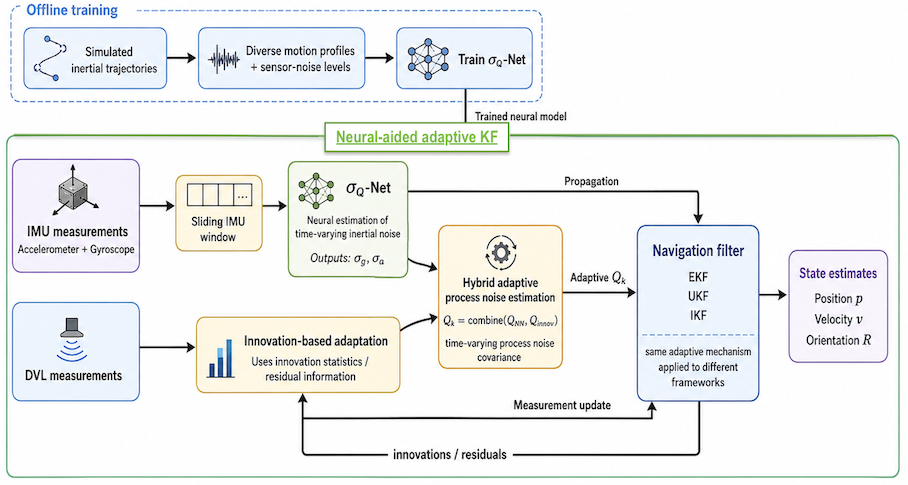
\includegraphics[width=\textwidth,height=6.0cm]{./SINNE_diag1.png}
    \caption{Common adaptive covariance-estimation mechanism used in the benchmark. A neural network estimates time-varying inertial sensor noise from a sliding IMU window, while an innovation-based adaptive mechanism extracts covariance information from the filter residuals. The two estimates are combined to construct the adaptive process noise covariance matrix $\mathbf{Q}_k$ used by the Neural-Aided EKF, Neural-Aided UKF, and Neural-Aided RI-IKF.}
    \label{propose_app}
\end{figure*}
\subsection{Neural-aided inertial learning approach}
The neural-learning-based approach in \cite{diker2026neural} maps a
window of recent inertial measurements to the gyroscope and
accelerometer process-noise parameters:
\begin{equation}
\boldsymbol{q}
=
f_{\theta}(\mathcal{W})
=
\begin{bmatrix}
\boldsymbol{q}_{g} \\
\boldsymbol{q}_{a}
\end{bmatrix}
\in \mathbb{R}^{6},
\end{equation}
%
where \(f_{\theta}\) denotes the neural network, \(\mathcal{W}\) is a
window of recent inertial measurements, and
\(\boldsymbol{q}_{g},\boldsymbol{q}_{a}\in\mathbb{R}^{3}\) contain
the predicted process-noise variances of the gyroscope and
accelerometer, respectively.
The continuous-time process-noise covariance matrix is then defined as
\begin{equation}
\mathbf{Q}_{c,\mathrm{neural}}
=
\operatorname{diag}
\left(
\boldsymbol{q}_{g},
\boldsymbol{q}_{a},
\boldsymbol{q}_{bg},
\boldsymbol{q}_{ba}
\right)
\in \mathbb{R}^{12 \times 12},
\end{equation}
%
where
\(\boldsymbol{q}_{bg}, \boldsymbol{q}_{ba} \in \mathbb{R}^{3}\)
represent the fixed gyroscope-bias and accelerometer-bias process-noise
variances, respectively. 
\subsection{Adaptive innovation model-based approach EKF/UKF}
The EKF and UKF require Euclidean innovation which is the difference between the DVL measurement and the estimated velocity in body frame which is
\begin{equation}
  \label{ekf_innovation}
  \nu_{innov} = v^b_{eb} - \hat{v}^b_{eb}
\end{equation}
where \(v^b_{eb}\) is the velocity expressed in the body frame as measured by the DVL and \(\hat{v}^b_{eb}\) is the estimated velocity expressed in the body. \\
The adaptive innovation-based process noise in steady state is given by \cite{mohamed1999adaptive} 
\begin{equation}
  \label{innovation_process_noise}
  \mathbf{Q}_{innov} = \frac{1}{N} \sum_{n=0}^N K_n \nu_n \nu^T_n K_n^T
\end{equation}
where \(\mathbf{K}_n\) is the Kalman gain at step \(n\) given by the EKF or the UKF, and \(\nu_n\) is the innovation.
\subsection{Adaptive innovation model-based approach RI-IKF}
\begin{comment}
While the EKF and UKF has difference between the prior and the posterior is given by
\begin{equation}
x - \hat{x} = K \nu 
\end{equation}
where \(\boldsymbol x\in \mathbb{R}^{15}\) is the posterior state, \(\hat{\boldsymbol x}\in\mathbb{R}^{15}\) is the prior state and \(\mathbf K\) is the Kalman gain. \\
The RI-IKF difference between the prior and posterior state is given by \eqref{RI-ikf_err} which is 
\begin{equation}
(\xi^R)^\wedge = log(\hat{\mathbf X}\mathbf X^{-1})
\end{equation}
where the function
\begin{equation}
  log(A)
=
\sum_{k=1}^{\infty}
\frac{(-1)^{k+1}}{k}(A-I)^k
\end{equation}
is a nonlinear mapping from the Lie group \(SE_2(3)\) into the Lie algebra \(\mathfrak{se}_2(3)\) and \(\mathbf X\) is given from \eqref{state_embbed} \\
\end{comment}
As shown in \cite{diker2026neural} the adaptive innovation-based process noise covariance that is derived from Lie innovation is
\begin{equation}
  \label{innov_RI-ikf}
\mathbf Q_{innov} = \frac{1}{N}\sum_{n=1}^N log(\hat{\mathbf X}\mathbf X^{-1})^{\vee} log(\hat{\mathbf X}\mathbf X^{-1})^{\vee,T} 
\end{equation}
where \(\mathbf X\) is the posterior state and \(\hat{\mathbf X}\) is the prior state and the mapping \((.)^{\vee}\) is given by the inverse of \eqref{vec2lie}
\begin{comment}
\begin{equation}
\begin{bmatrix}
0        & -\xi_3^R & \xi_2^R  & \xi_4^R & \xi_7^R \\
\xi_3^R  & 0        & -\xi_1^R & \xi_5^R & \xi_8^R \\
-\xi_2^R & \xi_1^R  & 0        & \xi_6^R & \xi_9^R \\
0        & 0        & 0        & 0        & 0       \\
0        & 0        & 0        & 0        & 0
\end{bmatrix}^{\vee}
=
\begin{bmatrix}
\xi_1^R \\
\xi_2^R \\
\xi_3^R \\
\xi_4^R \\
\xi_5^R \\
\xi_6^R \\
\xi_7^R \\
\xi_8^R \\
\xi_9^R
\end{bmatrix}
\end{equation}
\end{comment}
\subsection{Combined Process Noise Covariance}
Ultimately, The discrete-time process-noise covariance used by all Kalman filter variants is obtained by averaging the neural-network-based covariance and the adaptive innovation-based covariance:
\begin{equation}
\label{combined_process_noise}
\mathbf{Q}_{d}
=
\frac{1}{2}
\left(
\mathbf{G}\mathbf{Q}_{c,\mathrm{neural}}\mathbf{G}^{\mathsf{T}}
+
\mathbf{Q}_{d,\mathrm{innovation}}
\right)
\end{equation}
where the neural process noise covariance \(\mathbf{Q}_{c,\mathrm{neural}}\) is obtained by the same neural network with the same weights in all neural-aided Kalman filters. The innovation based covariance in neural-aided EKF and neural-aided UKF is given by \eqref{innovation_process_noise} and the innovation based covariance \(\mathbf{Q}_{d,\mathrm{innovation}}\) in neural-aided RI-IKF is given by \eqref{innov_RI-ikf}.
\begin{comment}
In this paper we have compared between those 3 approaches to enable the underwater navigation engineer to select the most fited approach. 
Those estimator are adapted with innovation based technique and a neural based learning algorithm that given an inertial window output the process noise covariance. In order to ensure fair comparison each estimator uses adapt the process noise covariance by taking half of the innovation based process noise and half from the neural learning based approach. The neural learning based network is trained using sim2real and the same network with the same weights are deployed in each estimator EKF, UKF and RI-IKF. The adaptive    
\end{comment}
\begin{comment}
Table \ref{tab:neuralnetwork1} presents the architecture of the proposed HINCA-KF, which is designed to be both lightweight and computationally efficient.
\end{comment}
\begin{comment}
\begin{table}[!t]
\centering
\caption{Architecture of the proposed HINCA-KF.}
\setlength{\tabcolsep}{3pt}
\renewcommand{\arraystretch}{1.1}
\begin{tabular}{l c p{3.2cm}}
\hline
\textbf{Layer} & \textbf{Dim.} & \textbf{Details} \\
\hline
Conv1D    & 32  & $k=5$, BN, LeakyReLU \\
Conv1D    & 64  & $k=5$, BN, LeakyReLU \\
Conv1D    & 128 & $k=5$, BN, LeakyReLU \\
Mean Pool & 256 & Temporal average pooling \\
FC        & 128 & LeakyReLU, Dropout \\
FC        & 32  & LeakyReLU, Dropout \\
FC        & 6   & Softplus activation \\
\hline
\end{tabular}
\label{tab:neuralnetwork1}
\end{table}
\end{comment}
\section{Analysis and Results}
\label{sec:results}
\subsection{Test Dataset}
\noindent The dataset used for the evaluation of our results (test dataset) was acquired by the Snapir AUV during maneuvers in the Mediterranean Sea \cite{cohen2025adaptive}. with a total mission duration of 4,800 seconds. To ensure a consistent and controlled evaluation across all filtering frameworks, additional zero mean white Gaussian noise was injected into the inertial and DVL measurements. The accelerometer measurements were corrupted with zero mean white Gaussian noise with a standard deviation of $4\times10^{-3}\mathrm{m/s^2}$, the gyroscope measurements with a standard deviation of $1\times10^{-4}\mathrm{rad/s}$, and the DVL measurements with a standard deviation of $5\times10^{-3}\mathrm{m/s}$. The same noise realization and noise levels were applied consistently to all evaluated filtering methods to ensure a fair comparison. \\
\subsection{Benchmarked Filtering Approaches}
\noindent Six filtering approaches are included in the benchmark: three model-based nonlinear Kalman filters and their corresponding neural-aided adaptive variants. All approaches use the same inertial navigation dynamics in \eqref{dynamics_ode}, IMU and DVL measurements, initial conditions, measurement noise covariance, and evaluation trajectories. The model-based approaches use a fixed process noise covariance matrix, whereas the neural-aided approaches use the adaptive process noise covariance defined in \eqref{combined_process_noise}. The same neural network, trained weights, input window, and adaptation parameters are used for all three neural-aided approaches. \\
\noindent The six benchmarked approaches are:
\begin{enumerate}
\item \textbf{EKF}: The model-based extended Kalman filter based on the Euclidean error-state formulation defined in \eqref{ekf_state}, using a fixed process noise covariance matrix.
\item \textbf{Neural-Aided EKF}: The same EKF formulation with the fixed process noise covariance replaced by the adaptive covariance in \eqref{combined_process_noise}. Its innovation-based component is calculated using \eqref{innovation_process_noise}.
\item \textbf{UKF}: The model-based unscented Kalman filter \ref{ukf}, in which the nonlinear state and measurement models are propagated using sigma points, with a fixed process noise covariance matrix.
\item \textbf{Neural-Aided UKF}: The same UKF formulation with the adaptive process noise covariance in \eqref{combined_process_noise}. As in the Neural-Aided EKF, its innovation-based component is calculated using \eqref{innovation_process_noise}.
\item \textbf{RI-IKF}: The model-based right-invariant Kalman filter based on the Lie-group error representation in \eqref{RI-ikf_err}, using a fixed process noise covariance matrix.
\item \textbf{Neural-Aided RI-IKF}: The same RI-IKF formulation with the adaptive process noise covariance in \eqref{combined_process_noise}. Its innovation-based component is calculated in the Lie algebra using \eqref{innov_RI-ikf}.
\end{enumerate}
\noindent This configuration provides a common ground for assessing two effects: the performance differences among the EKF, UKF, and RI-IKF formulations and the improvement obtained by applying the same neural-aided adaptive covariance-estimation mechanism to each formulation. 
\subsection{Results}
\noindent The EKF, UKF, and RI-IKF, together with their neural-aided variants, are evaluated against the post-processed ground-truth (GT) solution. Table~\ref{tab:filter_results} compares all six filtering approaches. In this benchmark, the position, velocity, and yaw root mean square errors are calculated relative to the post-processed GT solution. As shown in the table, the neural-aided variants consistently outperform their conventional model-based counterparts across all metrics. Notably, the Neural-Aided RI-IKF achieves the highest overall accuracy, yielding the lowest position error (7.61 m), velocity error (0.17 m/s), and yaw error (3.32$^\circ$). Furthermore, while all neural frameworks demonstrate a significant reduction in position drift, the invariant formulation leverages the adaptive process noise most effectively.
\begin{table}[h!]
\centering
\caption{Average navigation errors over 12 AUV trajectories.}
\begin{tabular}{|l|c|c|c|}
\hline
\textbf{Method} & \textbf{PRMSE [m]} & \textbf{VRMSE [m/s]} & \textbf{YRMSE [deg]} \\
\hline
EKF & 25.71 & 0.22 & 3.85 \\
\hline
Neural EKF & 17.80 & 0.18 & 3.44 \\
\hline
UKF & 27.51 & 0.25 & 4.01 \\
\hline
Neural UKF & 13.21 & 0.18 & 3.52 \\
\hline
RI-IKF & 21.64 & 0.24 & 3.42 \\
\hline
Neural RI-IKF & \textbf{7.61} & \textbf{0.17} & \textbf{3.32} \\
\hline
\end{tabular}
\label{tab:filter_results}
\end{table}
\noindent Figure~\ref{his_prmse} presents the PRMSE comparison for all six methods. These results indicate that the invariant formulation obtains the largest positioning benefit from the common adaptive covariance-estimation mechanism. As visually demonstrated in the chart, the integration of the neural-aided mechanism yields a distinct, stepped reduction in positioning drift for each filter. While the Neural-Aided EKF and Neural-Aided UKF reduce position errors by 30.8\% and 52.0\% respectively compared to their model-based baselines, the visualization highlights the superior adaptation of the Neural-Aided RI-IKF. It achieves a 64.8\% error reduction compared to its conventional counterpart, vastly outperforming the relative gains observed in the other frameworks. 
\begin{comment}
\noindent The neural-aided variants also reduce VRMSE by $18.2\%$, $28.0\%$, and $29.2\%$ for the EKF, UKF, and RI-IKF, respectively. The corresponding YRMSE reductions are $10.6\%$, $12.2\%$, and $2.9\%$. Although the heading improvement is relatively small for the RI-IKF, both its conventional and neural-aided variants provide the lowest heading errors among the compared approaches. Figure~\ref{his_prmse} presents the PRMSE comparison for all six methods. \\
\end{comment}
\begin{figure}[h!]
\centering
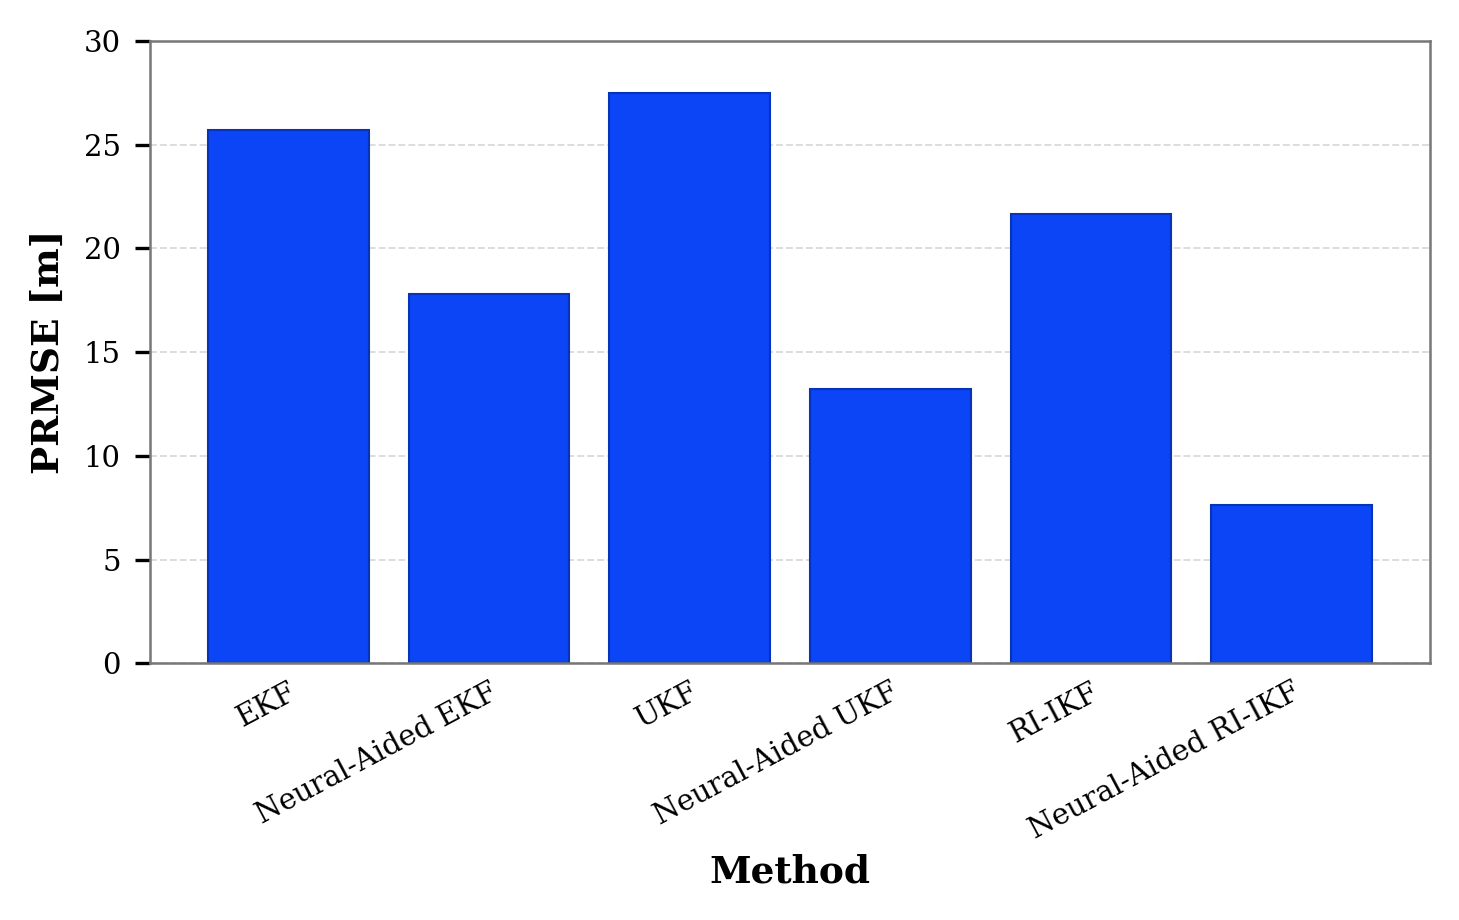
\includegraphics[height=5cm,width=1\linewidth]{./prmse_neural_aided.png}
\caption{PRMSE comparison of the EKF, UKF, and RI-IKF and their neural-aided variants.}
\label{his_prmse}
\end{figure}
\section{Conclusion}
\label{sec:conclusion}
\noindent This paper presented a common-ground benchmark of the EKF, UKF, RI-IKF, and their neural-aided adaptive variants using 12 real-world AUV trajectories totaling 4,800 seconds. All approaches were evaluated under identical sensor, noise, initialization, and adaptation conditions. Relative to their fixed-covariance counterparts, the Neural-Aided EKF, Neural-Aided UKF, and Neural-Aided RI-IKF reduced the position RMSE by $30.8\%$, $52.0\%$, and $64.8\%$, respectively. \\
\noindent The Neural-Aided RI-IKF achieved the best performance, reducing the position RMSE by $42.4\%$ relative to the Neural-Aided UKF and by $57.2\%$ relative to the Neural-Aided EKF. These results demonstrate that the benefit of adaptive process noise estimation depends on the underlying filtering formulation and that, under the evaluated of AUV navigation, the invariant formulation benefits most from the common adaptation mechanism. 
\begin{comment}
\section{Conclusion}
\label{sec:conclusion}
\noindent This paper presented HINCA-KF, a hybrid adaptive navigation framework that combines innovation-based covariance adaptation with neural estimation of time-varying inertial sensor noise. The proposed method was incorporated into three nonlinear filtering frameworks, resulting in HINCA-EKF, HINCA-UKF, and HINCA-RI-IKF. This formulation enabled a direct comparison of how different Kalman filtering approaches benefit from the same adaptive process noise covariance estimation mechanism. \\
\noindent The proposed approaches were evaluated on 12 real-world AUV trajectories collected in the Mediterranean Sea, with a total navigation duration of 4,800 seconds. To provide a controlled and consistent comparison, additional white noise was applied to the inertial and DVL measurements, and identical noise conditions were used for all evaluated filtering frameworks. The experimental results demonstrated that adaptive process noise estimation improves the position accuracy of all three filtering approaches. Compared with their corresponding fixed-covariance baselines, HINCA reduced the mean position RMSE by approximately $30.8\%$, $52.0\%$, and $64.8\%$ for the EKF, UKF, and IKF, respectively.\\
\noindent Among the evaluated methods, HINCA-IKF achieved the best overall navigation performance. In particular, its mean position RMSE was reduced by $42.4\%$ relative to HINCA-UKF and by $57.2\%$ relative to HINCA-EKF. The results therefore indicate that the benefit obtained from adaptive process noise estimation depends strongly on the underlying filtering formulation. In particular, the invariant error representation appears to provide a more suitable framework for exploiting time-varying covariance information in nonlinear inertial/DVL navigation. \\
\noindent These findings demonstrate that combining model-based innovation information with data-driven inertial noise estimation can substantially improve underwater navigation performance without restricting the adaptation mechanism to a particular Kalman filter formulation. Future work will investigate joint adaptation of the process and measurement noise covariance matrices, evaluate the proposed framework under additional vehicle dynamics and environmental conditions, and study its real-time implementation and computational requirements for onboard AUV navigation.
\end{comment}
\bibliographystyle{IEEEtran}
\bibliography{bio.bib}
\end{document}
